\pagebreak

\section{Resultados e Discussão}

Nesta seção, são apresentados os resultados obtidos para cada técnica de otimização aplicada, assim com os resultados do algoritmo sem otimização, será feito uma análise de speedup para cada técnica.

Para cada técnica, foi conduzida uma série de simulações utilizando combinações variadas de tamanhos de matriz e quantidades de iterações, conforme descrito a seguir:

\begin{itemize}
    \item \textbf{Tamanho da Matriz:} 2000, 4000, 6000
    \item \textbf{Quantidade de Iterações:} 500, 1000, 1500
\end{itemize}

Essas combinações foram escolhidas para simular diferentes cenários de complexidade computacional, permitindo uma análise detalhada do desempenho de cada técnica em condições variadas. Os resultados focam nas métricas de tempo de execução da simulação.

O ambiente de execução de todos os algoritmos (exceto do algoritmo em CUDA) tem as seguintes características:

\begin{itemize}
    \item Máquina: Notebook IdeaPad Lenovo
    \item CPU: Ryzen 5 5600G
    \item Memória RAM: 12 GB
    \item Compilador: GCC
\end{itemize}
\subsection{Resultados do Algoritmo Compilado com a Flag -O3}

\begin{figure}[H]
    \centering
    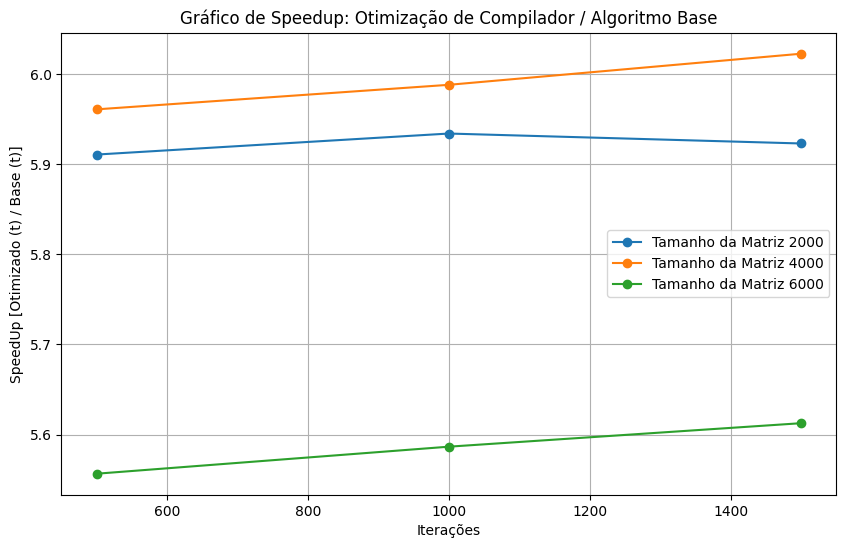
\includegraphics[width=1\linewidth]{../assets/O3 - SpeedUp.png}
\end{figure}

\subsection{Resultados do Algoritmo Paralelizado com OpenMP}

No gráfico abaixo, sobre a média de SpeedUp, os dois casos com o melhor SpeedUp é com 12 e 6 threads, invés de ser 12 e 10 threads, apesar de não ser encontrado um motivo para isso, pode ser que na configuração de 6 processos tem o menor overhead em comparação ao tempo ganho com a paralelização.

\begin{figure}[H]
    \centering
    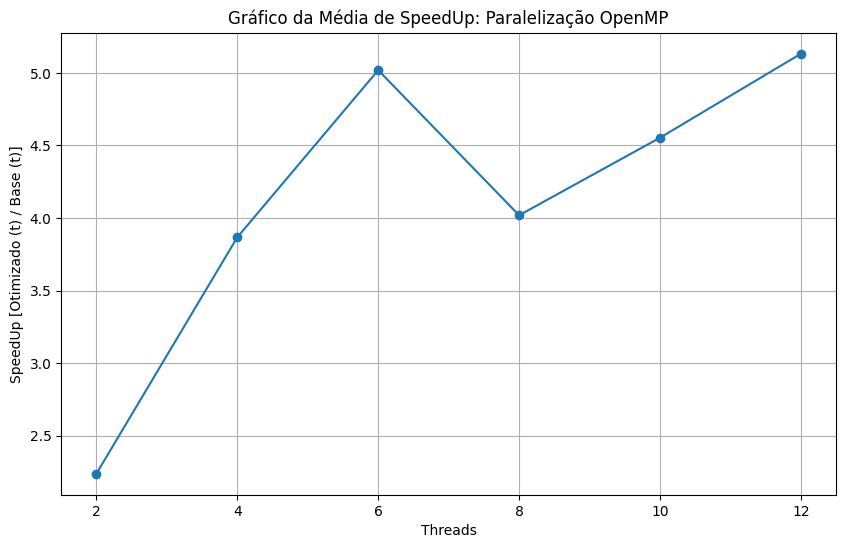
\includegraphics[width=1\linewidth]{../assets/OMP - SpeedUp.png}
\end{figure}

No gráfico abaixo, sobre a performance, é relevante a queda de performance conforme mais threads são usadas, indicando assim que quanto mais threads menos eficiente é o uso das CPUs.

\begin{figure}[H]
    \centering
    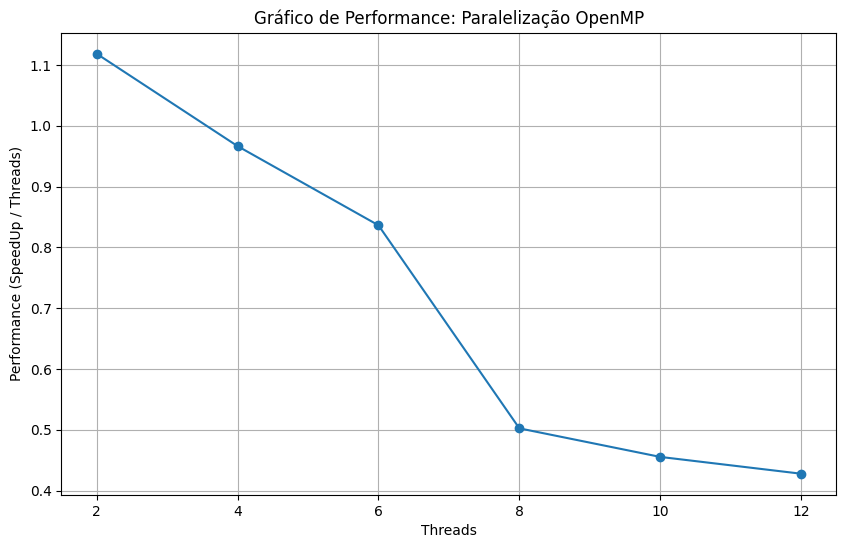
\includegraphics[width=1\linewidth]{../assets/OMP - Performance.png}
\end{figure}

\subsection{Resultados do Algoritmo Paralelizado com OpenMPI e com Otimização de Compilação}

No gráfico abaixo, sobre a média de SpeedUp, os dois casos com o melhor SpeedUp é com 6 (a melhor) e 10 processos, invés de ser 12 e 10 processos, isso pode ocorrer por diminuir a quantidade de sincronização necessária entre processos enquanto há uma divisão adequada de trabalho entre os processos.

\begin{figure}[H]
    \centering
    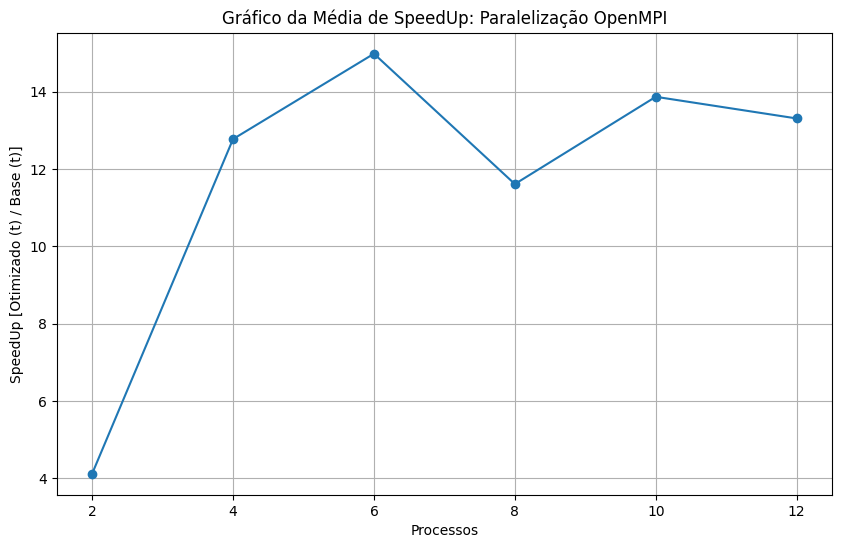
\includegraphics[width=1\linewidth]{../assets/MPI - SpeedUp.png}
\end{figure}

No gráfico abaixo, sobre a performance, é relevante notar que em comparação a paralelização com OpenOMP, a performance com MPI sempre está acima que 1, enquanto do OpenOMP esteve em sua maioria, abaixo de 1, assim indicando uma ótima utilização dos recursos do computador quando a atividade é dividida entre processos que em threads.

\begin{figure}[H]
    \centering
    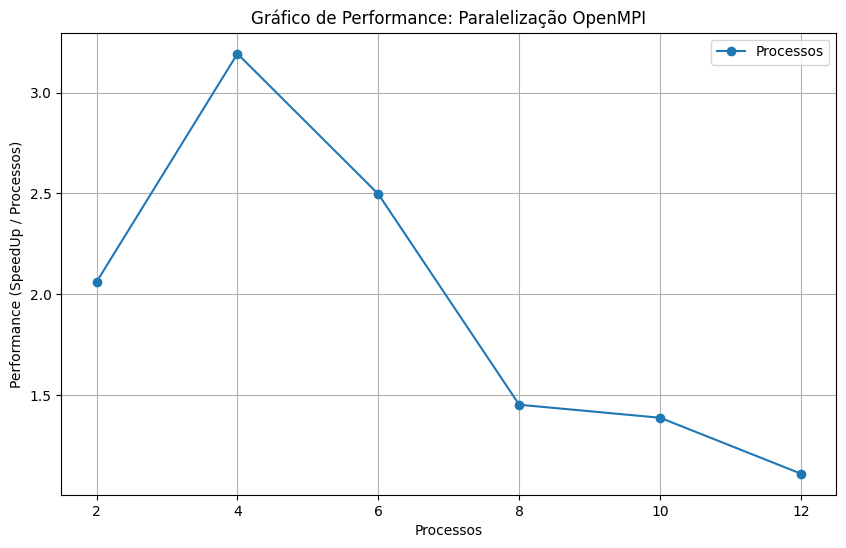
\includegraphics[width=1\linewidth]{../assets/MPI - Performance.png}
\end{figure}

\subsection{Resultados do Algoritmo Adaptado para CUDA}
\subsubsection{Configuração do Ambiente de Execução}
\begin{itemize}
    \item Máquina: Ambiente Virtual do Google Colab
    \item CPU:
    \item Memória RAM: 16 GB
    \item GPU: T4
    \item Compilador: NVCC (NVIDIA CUDA Compiler)
\end{itemize}

No gráfico abaixo de SpeedUp, comparando cada caso com um tamanho de bloco diferente, é notável que com 16 de tamanho de bloco é o que apresentou o melhor SpeedUp. Esse comportamento pode ser explicado pelo balanceamento entre a ocupação da GPU e a minimização da sobrecarga associada à troca de contexto entre warps. Blocos muito pequenos podem não explorar eficientemente a capacidade dos multiprocessadores da GPU, enquanto blocos muito grandes podem causar contenção de recursos e maior latência na comunicação entre threads.

\begin{figure}[H]
    \centering
    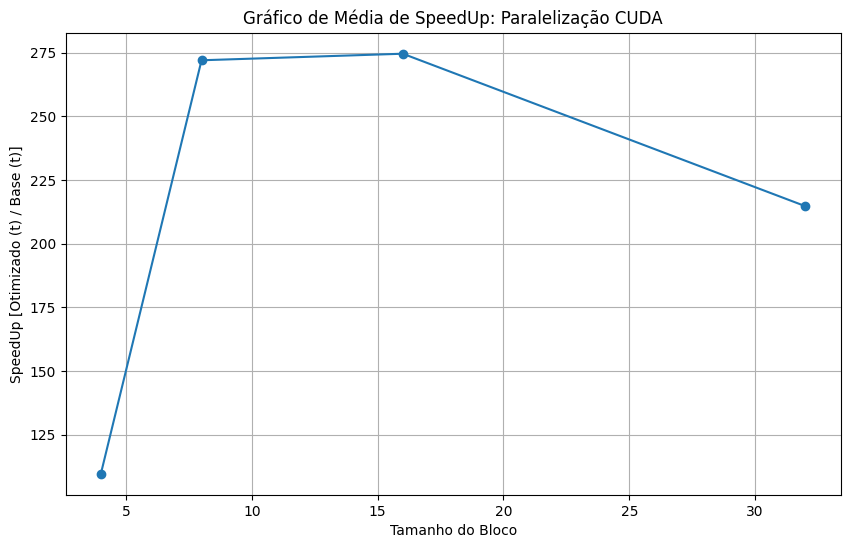
\includegraphics[width=1\linewidth]{../assets/CUDA - SpeedUp.png}
\end{figure}

\subsection{Comparativo com todos os Métodos}

\begin{figure}[H]
    \centering
    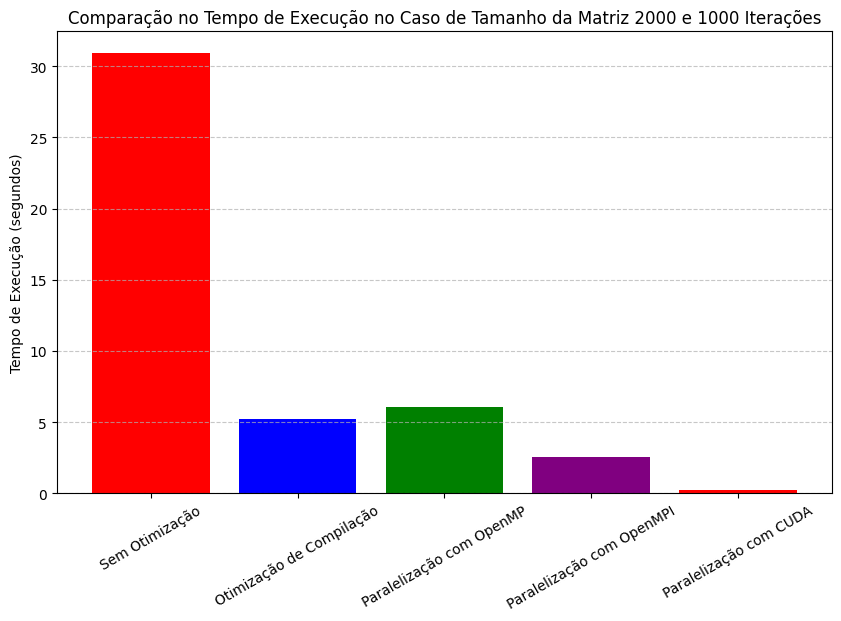
\includegraphics[width=1\linewidth]{../assets/Final.png}
\end{figure}

Os resultados obtidos evidenciam que a implementação CUDA apresentou o melhor desempenho, mas houve uma falha na obtenção de mais dados, o que limitou a análise mais aprofundada da escalabilidade da solução.

Entre as otimizações com CPU, OpenMPI apresentou o melhor resultado utilizando de 6 processos. E curiosamente, a versão sequencial otimizada com a flag -O3 do GCC superou a implementação OpenMP com 12 threads. Isso sugere que a otimização agressiva aplicada pelo compilador, foi suficiente para melhorar o desempenho sem a necessidade do overhead de gerenciamento de múltiplas threads, indicando que problemas de itensivo iteração pode ser otimizados em compilação.
